\chapter{Symmetric Cryptography and Hash Functions}\label{ch:b3:symmetric-cryptography}

Two parties who share a secret key want to talk over a network that anyone can read and anyone can tamper with. This chapter says first what ``secure'' should mean, proves that \omterm{def:b3:symmetric-cryptography:security}{perfect secrecy} exists and costs a key as long as the message, and then builds, from the published standards, the tools that real systems use instead: the \omterm{def:b3:symmetric-cryptography:block}{block cipher} \omterm{def:b3:symmetric-cryptography:block}{AES} and the ways to chain it, the \omterm{def:b3:symmetric-cryptography:stream}{stream cipher} ChaCha20, the hash function SHA-256, and the \omterm{def:b3:symmetric-cryptography:mac}{message authentication codes} that detect tampering. Every one is checked against its standard's test vectors, and every misuse that the chapter shows, a reused key, a \omterm{def:b3:symmetric-cryptography:modes}{padding} error message, a naive authentication tag, is an attack on the chapter's own toy services, followed by its fix. The programs are written to be read.

\begin{inpractice}[Use a vetted library]
A real system never runs code like this chapter's. It calls a vetted library, whose code has been reviewed for years, runs in constant time and is patched when an attack appears; Python's own \code{hashlib}, \code{hmac} and \code{secrets} cover hashing, MACs and key generation. The chapter's implementations are for understanding, and they are checked against the standards so that what they show is true.
\end{inpractice}

\begin{recall}
A cipher turns a plaintext into a ciphertext with a key; frequency analysis breaks a substitution cipher by counting letters (grade~9 volume), and a computer encrypts with standard ciphers and checks data with hash functions (grade~12 volume). XOR, $\oplus$, adds bits modulo 2, so $a \oplus b \oplus b = a$. In the mathematics books, the bytes form the finite field $\mathrm{GF}(2^8)$, polynomials over $\{0, 1\}$ modulo an irreducible one of degree 8, where every non-zero element has an inverse; and among 23 people, two share a birthday more often than not.
\end{recall}

\section{What ``secure'' means}\label{sec:b3:symmetric-cryptography:security}

\begin{definition}[Kerckhoffs's principle, attack model, perfect secrecy, computational security, indistinguishability]\label{def:b3:symmetric-cryptography:security}
\emph{Kerckhoffs's principle}\index{Kerckhoffs's principle} asks a cipher to stay secure when everything about it except the key is public. An \emph{attack model}\index{attack model} says what the attacker may do: see ciphertexts only; know some plaintexts and their ciphertexts; have plaintexts of its choice encrypted (chosen plaintext); or also have ciphertexts of its choice decrypted (chosen ciphertext). A cipher has \emph{perfect secrecy}\index{perfect secrecy} if, for a key chosen uniformly, every ciphertext is equally likely whatever the plaintext: $P(C = c \mid M = m) = P(C = c \mid M = m')$ for all $m$, $m'$, $c$. It has \emph{computational security}\index{computational security} if no attacker with a realistic amount of computation succeeds with more than a negligible probability. \emph{Indistinguishability}\index{indistinguishability} is the game that makes this precise: the attacker chooses two messages $m_0$, $m_1$ of the same length, receives the encryption of one of them, chosen by a fair coin, may go on using its attack model, and must guess which; the cipher is secure if no efficient attacker guesses right with probability noticeably above $1/2$.
\end{definition}

Kerckhoffs stated the principle in an article of 1883; Shannon, who put secrecy on a mathematical footing in 1949, phrased it as ``the enemy knows the system''. % ledger: b3:kerckhoffs-1883, b3:shannon-1949
A secret algorithm is found out sooner or later, by a stolen device or a leaked program; a key can be changed in a minute.

\begin{definition}[One-time pad]\label{def:b3:symmetric-cryptography:otp}
The \emph{one-time pad}\index{one-time pad} encrypts an $n$-byte message $m$ with a uniformly random $n$-byte key $k$, used for one message only: $c = m \oplus k$, and $m = c \oplus k$.
\end{definition}

\begin{theorem}[Shannon's secrecy theorem]\label{thm:b3:symmetric-cryptography:shannon}
The \omterm{def:b3:symmetric-cryptography:otp}{one-time pad} has \omterm{def:b3:symmetric-cryptography:security}{perfect secrecy}. Conversely, a cipher with \omterm{def:b3:symmetric-cryptography:security}{perfect secrecy} has at least as many keys as messages.\index{Shannon's secrecy theorem}
\end{theorem}

\begin{proof}
For the pad, given $m$ and $c$, exactly one key gives $c$, namely $k = m \oplus c$, so $P(C = c \mid M = m) = 2^{-8n}$, the same for every $m$. Conversely, take a ciphertext $c$ that occurs, from some message $m_0$ and some key. By \omterm{def:b3:symmetric-cryptography:security}{perfect secrecy}, $P(C = c \mid M = m) = P(C = c \mid M = m_0) > 0$ for every message $m$, so for each $m$ some key encrypts $m$ to $c$. Decryption with a key is a function of $c$, so one key cannot decrypt $c$ to two different messages: these keys are all different, and there are at least as many keys as messages.
\end{proof}

The price is a key as long as everything ever sent, delivered in advance and never reused. Reuse is fatal: if $c_1 = m_1 \oplus k$ and $c_2 = m_2 \oplus k$, then $c_1 \oplus c_2 = m_1 \oplus m_2$, the key is gone, and a guessed word in one message reveals the other at the same place.

\omcode{code/bachelor-3/27-symmetric-cryptography/listings/otp.py}{1}{27}{A \omterm{def:b3:symmetric-cryptography:otp}{one-time pad}, a key that turns the same ciphertext into any other message of the same length, and a key used twice.}\label{lst:b3:symmetric-cryptography:otp}

\omoutput{code/bachelor-3/27-symmetric-cryptography/outputs/otp.txt}{Guessing ``THE '' at position 0 gives MEET, which reads like text: a hit, THE starts one message and MEET the other. LIBRARY at 12 gives NDER TH.}\label{out:b3:symmetric-cryptography:otp}

The key here comes from \code{random} with a seed, so that the run repeats. Python's documentation says that \code{random} is designed for modelling and simulation, and that real keys come from \code{secrets}. % ledger: b3:py-crypto-docs
The rest of the chapter gives up \omterm{def:b3:symmetric-cryptography:security}{perfect secrecy} for \omterm{def:b3:symmetric-cryptography:security}{computational security}: a 16-byte key that encrypts gigabytes, secure as long as no one can do much better than trying the $2^{128}$ keys.

\section{Block ciphers and their modes}\label{sec:b3:symmetric-cryptography:block}

\begin{definition}[Block cipher, round key, AES]\label{def:b3:symmetric-cryptography:block}
A \emph{block cipher}\index{block cipher} is a family of permutations of the $n$-bit blocks, one for each key, $E_k$, with an inverse $D_k$ that is efficient to compute when $k$ is known. Most are built from rounds, each mixing the block with a \emph{round key}\index{round key} derived from the key. \emph{AES}\index{AES} is the block cipher of the standard FIPS 197: 16-byte blocks, keys of 16, 24 or 32 bytes, and 10, 12 or 14 rounds.
\end{definition}

\omterm{def:b3:symmetric-cryptography:block}{AES} treats the block as a $4 \times 4$ array of bytes. Each round applies four steps: SubBytes replaces every byte by its inverse in $\mathrm{GF}(2^8)$ followed by a fixed affine map, the only non-linear step; ShiftRows rotates row $r$ by $r$ places; MixColumns multiplies every column by a fixed matrix over $\mathrm{GF}(2^8)$, so that each output byte depends on the whole column; AddRoundKey XORs the \omterm{def:b3:symmetric-cryptography:block}{round key}. Two rounds of ShiftRows and MixColumns already make every byte of the state depend on every byte of the input. % ledger: b3:aes-fips197

\begin{omfigure}
\begin{tikzpicture}[font=\small, node distance=0.55cm, st/.style={draw, rounded corners=2pt, minimum width=2.7cm, minimum height=0.62cm, fill=omDef!8}, ar/.style={-{Stealth}, thick}]
  \node (in) {state, 16 bytes};
  \node[st, below=of in] (sb) {SubBytes};
  \node[st, below=of sb] (sr) {ShiftRows};
  \node[st, below=of sr] (mc) {MixColumns};
  \node[st, below=of mc, fill=omThm!10] (ak) {AddRoundKey};
  \node[below=of ak] (out) {state};
  \node[left=1.2cm of ak] (k) {round key $k_r$};
  \foreach \a/\b in {in/sb, sb/sr, sr/mc, mc/ak, ak/out} \draw[ar] (\a) -- (\b);
  \draw[ar] (k) -- (ak);
  \node[right=0.4cm of sb, align=left, font=\footnotesize] {each byte $b \mapsto$ affine$(b^{-1})$ in $\mathrm{GF}(2^8)$};
  \node[right=0.4cm of sr, align=left, font=\footnotesize] {row $r$ rotated $r$ places left};
  \node[right=0.4cm of mc, align=left, font=\footnotesize] {each column times a fixed matrix\\ (left out in the last round)};
  \node[right=0.4cm of ak, align=left, font=\footnotesize] {XOR with 16 bytes from the key};
\end{tikzpicture}
\par\smallskip{\small One round of \omterm{def:b3:symmetric-cryptography:block}{AES}. AES-128 adds \omterm{def:b3:symmetric-cryptography:block}{round key} $k_0$ first, then runs ten rounds with $k_1$ to $k_{10}$.}
\end{omfigure}

\omcode{code/bachelor-3/27-symmetric-cryptography/listings/aes.py}{93}{101}{AES-128 encryption: the initial key addition, nine full rounds, and a last round without MixColumns.}\label{lst:b3:symmetric-cryptography:aes}

\omoutput{code/bachelor-3/27-symmetric-cryptography/outputs/aes_vector.txt}{The cipher example of FIPS 197: the S-box, two \omterm{def:b3:symmetric-cryptography:block}{round keys} and the ciphertext agree with the standard, and decryption gives the plaintext back.}\label{out:b3:symmetric-cryptography:aes}

A \omterm{def:b3:symmetric-cryptography:block}{block cipher} encrypts 16 bytes. A message is longer, and its length is rarely a multiple of 16.

\begin{definition}[Mode of operation, ECB, CBC, initialisation vector, padding, CTR, padding oracle]\label{def:b3:symmetric-cryptography:modes}
A \emph{mode of operation}\index{mode of operation} encrypts a message of several blocks $P_1, \ldots, P_n$ with a \omterm{def:b3:symmetric-cryptography:block}{block cipher}. \emph{ECB mode}\index{ECB mode} encrypts each block alone: $C_i = E_k(P_i)$. \emph{CBC mode}\index{CBC mode} chains them: $C_i = E_k(P_i \oplus C_{i-1})$, starting from $C_0$, an \emph{initialisation vector}\index{initialisation vector} (IV) that must be unpredictable and is sent with the ciphertext; decryption computes $P_i = D_k(C_i) \oplus C_{i-1}$. \emph{Padding}\index{padding} extends the message to a whole number of blocks; PKCS\#7 padding adds $p$ bytes of value $p$, $1 \le p \le 16$, and is checked and removed after decryption. \emph{CTR mode}\index{CTR mode} turns the \omterm{def:b3:symmetric-cryptography:block}{block cipher} into a \omterm{def:b3:symmetric-cryptography:stream}{stream cipher}: $C_i = P_i \oplus E_k(\mathit{ctr} + i)$, with a counter block that must never repeat under one key. A \emph{padding oracle}\index{padding oracle} is any way for an attacker to learn whether the padding of a ciphertext of its choice was valid. % ledger: b3:sp800-38a
\end{definition}

NIST's SP 800-38A defines ECB, CBC and CTR, among five modes, with test vectors that the chapter's tests check. % ledger: b3:sp800-38a
ECB is a code book: equal plaintext blocks give equal ciphertext blocks. A picture shows it. The program below draws a ring and a bar, one byte per pixel, and encrypts it in both modes.

\omoutput{code/bachelor-3/27-symmetric-cryptography/outputs/ecb_pattern.txt}{The picture has 384 blocks, only 41 of them different: ECB keeps exactly 41, CBC gives 384 different blocks.}\label{out:b3:symmetric-cryptography:ecb}

\begin{omfigure}
\centering
\begin{tikzpicture}
  \begin{axis}[width=0.36\linewidth, height=0.3\linewidth, scale only axis=false, axis equal image, hide axis, colormap/blackwhite, enlargelimits=false, title style={font=\small}, title={plaintext}]
    \addplot[matrix plot*, mesh/cols=96, point meta=explicit] table[x=x, y=y, meta=plain] {code/bachelor-3/27-symmetric-cryptography/figures/ecb.dat};
  \end{axis}
\end{tikzpicture}\hfill
\begin{tikzpicture}
  \begin{axis}[width=0.36\linewidth, height=0.3\linewidth, scale only axis=false, axis equal image, hide axis, colormap/blackwhite, enlargelimits=false, title style={font=\small}, title={ECB}]
    \addplot[matrix plot*, mesh/cols=96, point meta=explicit] table[x=x, y=y, meta=ecb] {code/bachelor-3/27-symmetric-cryptography/figures/ecb.dat};
  \end{axis}
\end{tikzpicture}\hfill
\begin{tikzpicture}
  \begin{axis}[width=0.36\linewidth, height=0.3\linewidth, scale only axis=false, axis equal image, hide axis, colormap/blackwhite, enlargelimits=false, title style={font=\small}, title={CBC}]
    \addplot[matrix plot*, mesh/cols=96, point meta=explicit] table[x=x, y=y, meta=cbc] {code/bachelor-3/27-symmetric-cryptography/figures/ecb.dat};
  \end{axis}
\end{tikzpicture}
\par\smallskip{\small A picture of $96 \times 64$ one-byte pixels, drawn from \code{figures/ecb.dat}, encrypted with AES-128. In ECB each run of 16 equal pixels becomes the same 16 bytes, and the shapes stay visible; in CBC the ciphertext looks random.}
\end{omfigure}

\omcode{code/bachelor-3/27-symmetric-cryptography/listings/modes.py}{34}{39}{CBC encryption: each block is XORed with the previous ciphertext block, the first with the IV, before it is encrypted.}\label{lst:b3:symmetric-cryptography:cbc}

\begin{omfigure}
\begin{tikzpicture}[font=\small, x=1.9cm, y=1cm, bc/.style={draw, fill=omDef!10, minimum width=1cm, minimum height=0.6cm}, xo/.style={circle, draw, inner sep=0pt, minimum size=0.36cm}, ar/.style={-{Stealth}, thick}]
  \node at (-0.7,2.4) {CBC};
  \node (iv) at (-0.4,1.1) {IV};
  \foreach \i in {1,2,3} {
    \node (p\i) at (\i,2.4) {$P_\i$};
    \node[xo] (x\i) at (\i,1.7) {$+$};
    \node[bc] (e\i) at (\i,0.9) {$E_k$};
    \node (c\i) at (\i,0.0) {$C_\i$};
    \draw[ar] (p\i) -- (x\i); \draw[ar] (x\i) -- (e\i); \draw[ar] (e\i) -- (c\i);
  }
  \draw[ar] (iv) |- (x1);
  \draw[ar] (e1.south) ++(0,-0.2) -| ++(0.5,0) |- (x2);
  \draw[ar] (e2.south) ++(0,-0.2) -| ++(0.5,0) |- (x3);
  \begin{scope}[xshift=7.6cm]
  \node at (0.3,2.4) {CTR};
  \foreach \i/\c in {1/{ctr}, 2/{ctr+1}, 3/{ctr+2}} {
    \node (n\i) at (\i,2.4) {$\mathit{\c}$};
    \node[bc] (f\i) at (\i,1.6) {$E_k$};
    \node[xo] (y\i) at (\i,0.75) {$+$};
    \node (q\i) at (\i-0.45,0.75) {$P_\i$};
    \node (d\i) at (\i,0.0) {$C_\i$};
    \draw[ar] (n\i) -- (f\i); \draw[ar] (f\i) -- (y\i); \draw[ar] (q\i) -- (y\i); \draw[ar] (y\i) -- (d\i);
  }
  \end{scope}
\end{tikzpicture}
\par\smallskip{\small Two modes. In CBC each ciphertext block feeds the next encryption, so equal plaintext blocks encrypt differently, and encryption is sequential. In CTR the cipher only produces a \omterm{def:b3:symmetric-cryptography:stream}{keystream} from the counter, and the blocks can be computed in parallel; a repeated counter repeats the \omterm{def:b3:symmetric-cryptography:stream}{keystream}.}
\end{omfigure}

CBC hides patterns but not errors. The receiver decrypts, then checks the \omterm{def:b3:symmetric-cryptography:modes}{padding}, and a service that answers differently to bad \omterm{def:b3:symmetric-cryptography:modes}{padding} than to other errors gives the attacker one bit per query: is the last byte of $D_k(C) \oplus C'$ a valid \omterm{def:b3:symmetric-cryptography:modes}{padding}, for a forged block $C'$ of the attacker's choice? Vaudenay described in 2002 how this bit decrypts the whole message. % ledger: b3:vaudenay-2002
The attacker changes the last byte of $C'$ until the \omterm{def:b3:symmetric-cryptography:modes}{padding} is valid: then the last byte of $D_k(C) \oplus C'$ is \code{01}, which gives the last byte of $D_k(C)$, and XORed with the real previous block, the plaintext's. Then it aims for \code{02 02}, and so on, at most 256 queries per byte.

\omcode{code/bachelor-3/27-symmetric-cryptography/listings/padding_oracle.py}{28}{44}{One block of the attack: find $D_k(C)$ byte by byte from the end, forging the block before it so that the known bytes decrypt to the \omterm{def:b3:symmetric-cryptography:modes}{padding} sought.}\label{lst:b3:symmetric-cryptography:oracle}

\omoutput{code/bachelor-3/27-symmetric-cryptography/outputs/padding_oracle.txt}{Three blocks recovered in 6,389 queries, without the key. When the service checks an \omterm{def:b3:symmetric-cryptography:mac}{HMAC} over the ciphertext before decrypting, the same 12,288 forged queries are all refused and reveal nothing.}\label{out:b3:symmetric-cryptography:oracle}

The fix is not a better error message but authentication: a service that rejects every ciphertext it did not produce, before decrypting it, has nothing to leak. The last section builds it.

\section{Stream ciphers}\label{sec:b3:symmetric-cryptography:stream}

\begin{definition}[Stream cipher, keystream, nonce]\label{def:b3:symmetric-cryptography:stream}
A \emph{stream cipher}\index{stream cipher} expands a short key into a long pseudo-random \emph{keystream}\index{keystream} and XORs it with the message, as a \omterm{def:b3:symmetric-cryptography:otp}{one-time pad} with a computed key. A \emph{nonce}\index{nonce} (number used once) is an input that makes the keystream differ from message to message under the same key; a nonce must never be reused with the same key.
\end{definition}

A reused \omterm{def:b3:symmetric-cryptography:stream}{nonce} is a reused pad, with the leak of \cref{out:b3:symmetric-cryptography:otp}. ChaCha20, designed by Bernstein and specified in RFC 8439, makes 64 bytes of \omterm{def:b3:symmetric-cryptography:stream}{keystream} from a 32-byte key, a 32-bit block counter and a 12-byte \omterm{def:b3:symmetric-cryptography:stream}{nonce}. % ledger: b3:rfc8439
Its state is sixteen 32-bit words: four constants, the key, the counter and the \omterm{def:b3:symmetric-cryptography:stream}{nonce}. Twenty rounds of additions, XORs and rotations mix them, and the initial state is added back at the end, so that the rounds cannot simply be run backwards from the output.

\omcode{code/bachelor-3/27-symmetric-cryptography/listings/chacha20.py}{13}{41}{The quarter round, and the block function: ten double rounds, four on the columns of the $4 \times 4$ state and four on its diagonals.}\label{lst:b3:symmetric-cryptography:chacha}

\omoutput{code/bachelor-3/27-symmetric-cryptography/outputs/chacha20.txt}{The two test vectors of RFC 8439, sections 2.3.2 and 2.4.2, reproduced.}\label{out:b3:symmetric-cryptography:chacha}

ChaCha20 uses only additions, XORs and rotations of words, which take the same time whatever their values; table look-ups such as \omterm{def:b3:symmetric-cryptography:block}{AES}'s S-box can take a time that depends on the key through the cache, and RFC 8439 notes that many \omterm{def:b3:symmetric-cryptography:block}{AES} implementations are open to such timing attacks. % ledger: b3:rfc8439

\section{Hash functions}\label{sec:b3:symmetric-cryptography:hash}

\begin{definition}[Cryptographic hash function, preimage resistance, second-preimage resistance, collision resistance]\label{def:b3:symmetric-cryptography:hash}
A \emph{cryptographic hash function}\index{cryptographic hash function} maps messages of any length to a fixed-length digest, computed by a public algorithm, with no key. It has \emph{preimage resistance}\index{preimage resistance} if, given a digest $h$, finding any $m$ with $H(m) = h$ is infeasible; \emph{second-preimage resistance}\index{second-preimage resistance} if, given $m$, finding $m' \ne m$ with $H(m') = H(m)$ is infeasible; and \emph{collision resistance}\index{collision resistance} if finding any two different messages with the same digest is infeasible.
\end{definition}

A hash table needs a hash function that spreads keys well; a cryptographic one must also resist an adversary who chooses the inputs (Year~1 volume). Collisions exist, since there are more messages than digests; resistance means they are hard to find. And they are easier to find than preimages, by the same count that makes shared birthdays common.

\begin{theorem}[Birthday bound]\label{thm:b3:symmetric-cryptography:birthday}
Draw $q$ values independently and uniformly from a set of $N$. The probability that all are different is at most $e^{-q(q-1)/(2N)}$. So $q \approx \sqrt{2N \ln 2} \approx 1.18\sqrt{N}$ draws give a collision with probability at least $1/2$.\index{birthday bound}
\end{theorem}

\begin{proof}
Facts used: $1 - x \le e^{-x}$ for every real $x$. The $i$-th draw, $i = 1, \ldots, q$, avoids the $i - 1$ earlier values, all different, with probability $1 - (i - 1)/N$, so
\[ P(\text{all different}) = \prod_{i=1}^{q} \Bigl(1 - \frac{i - 1}{N}\Bigr) \le \prod_{i=1}^{q} e^{-(i-1)/N} = e^{-q(q - 1)/(2N)}. \]
This is at most $1/2$ as soon as $q(q - 1) \ge 2N \ln 2$, which holds for $q = \lceil \sqrt{2N \ln 2}\, \rceil + 1$.
\end{proof}

A finer computation gives the mean number of draws until the first collision, about $\sqrt{\pi N / 2}$. A digest of $b$ bits therefore resists collisions for only about $2^{b/2}$ work: the 256 bits of SHA-256 give $2^{128}$. The weekend problem measures the bound on a 32-bit digest.

\begin{definition}[Merkle--Damgård construction, length-extension attack]\label{def:b3:symmetric-cryptography:md}
The \emph{Merkle--Damgård construction}\index{Merkle--Damgård construction} hashes a message by \omterm{def:b3:symmetric-cryptography:modes}{padding} it to whole blocks, with its length in the last one, and running a compression function $f$ along the blocks: $h_0$ is a fixed initial value, $h_i = f(h_{i-1}, M_i)$, and the digest is $h_n$. A \emph{length-extension attack}\index{length-extension attack} uses $H(m)$ and the length of $m$, without $m$, to compute $H(m \,\|\, \mathit{pad} \,\|\, m')$ for any $m'$, by continuing the chain from $h_n$.
\end{definition}

SHA-256, from FIPS 180-4, is a \omterm{def:b3:symmetric-cryptography:md}{Merkle--Damgård construction} with 64-byte blocks and a 32-byte state. Its 64 round constants are the first 32 bits of the fractional parts of the cube roots of the first 64 primes, and its initial value comes from the square roots of the first 8: numbers anyone can recompute, rather than numbers the designers picked. % ledger: b3:fips180-sha256

\omcode{code/bachelor-3/27-symmetric-cryptography/listings/sha256.py}{49}{66}{The compression function of SHA-256: a message schedule of 64 words, then 64 rounds over eight working words, added to the previous state.}\label{lst:b3:symmetric-cryptography:sha}

\omoutput{code/bachelor-3/27-symmetric-cryptography/outputs/sha256_check.txt}{The constants agree with FIPS 180-4, and the digests with Python's \code{hashlib} on 1,000 random messages. A message of 56 bytes needs a second block: its 8-byte length no longer fits.}\label{out:b3:symmetric-cryptography:sha}

\begin{omfigure}
\begin{tikzpicture}[font=\small, x=1.75cm, f/.style={draw, fill=omDef!10, minimum width=0.8cm, minimum height=0.65cm}, ar/.style={-{Stealth}, thick}]
  \node (h0) at (0,0) {$h_0$};
  \foreach \i/\l in {1/{k\,\|\,m_1}, 2/{m_2}, 3/{m_3\,\|\,\mathit{pad}}} {
    \node[f] (f\i) at (\i,0) {$f$};
    \node (m\i) at (\i,1.1) {$\l$};
    \draw[ar] (m\i) -- (f\i);
  }
  \draw[ar] (h0) -- (f1); \draw[ar] (f1) -- (f2); \draw[ar] (f2) -- (f3);
  \node (t) at (4,0) {$h_3 = $ tag};
  \draw[ar] (f3) -- (t);
  \node[f, fill=omThm!12] (f4) at (5.2,0) {$f$};
  \node (m4) at (5.2,1.1) {$m' \,\|\, \mathit{pad}'$};
  \draw[ar, omThm] (t) -- (f4); \draw[ar, omThm] (m4) -- (f4);
  \node (t2) at (6.3,0) {new tag};
  \draw[ar, omThm] (f4) -- (t2);
  \draw[decorate, decoration={brace, amplitude=5pt, mirror}] (0.7,-0.6) -- (3.3,-0.6) node[midway, below=6pt] {the service, with the key $k$};
  \draw[decorate, decoration={brace, amplitude=5pt, mirror}, omThm] (4.7,-0.6) -- (5.7,-0.6) node[midway, below=6pt] {the attacker};
\end{tikzpicture}
\par\smallskip{\small The Merkle--Damgård chain of $H(k \,\|\, m)$, and its continuation. The tag is the whole state after the last block, so anyone who knows it can hash further blocks; the result is the tag of $k \,\|\, m \,\|\, \mathit{pad} \,\|\, m'$.}
\end{omfigure}

\section{Message authentication}\label{sec:b3:symmetric-cryptography:mac}

\begin{definition}[Message authentication code, HMAC, authenticated encryption, AEAD]\label{def:b3:symmetric-cryptography:mac}
A \emph{message authentication code}\index{message authentication code} (MAC) computes, from a key and a message, a tag that no one without the key can compute for a new message, even after seeing the tags of messages of its choice. \emph{HMAC}\index{HMAC} is the MAC of RFC 2104 built from a hash function $H$ with blocks of $B$ bytes: $\mathrm{HMAC}(K, m) = H\bigl((K \oplus \mathit{opad}) \,\|\, H((K \oplus \mathit{ipad}) \,\|\, m)\bigr)$, where the key is padded with zeros to $B$ bytes and $\mathit{ipad}$, $\mathit{opad}$ are the bytes \code{0x36} and \code{0x5C} repeated $B$ times. \emph{Authenticated encryption}\index{authenticated encryption} gives both secrecy and integrity: the receiver either gets the plaintext or learns that the ciphertext was changed. \emph{AEAD}\index{AEAD} (authenticated encryption with associated data) also authenticates data sent in the clear, such as a header.
\end{definition}

The tempting MAC $H(k \,\|\, m)$ falls to length extension. A toy library service authorises loans with such tags:

\omcode{code/bachelor-3/27-symmetric-cryptography/listings/length_ext.py}{19}{30}{Forging a tag for a longer order: continue SHA-256 from the published tag, after the \omterm{def:b3:symmetric-cryptography:modes}{padding} the service itself added.}\label{lst:b3:symmetric-cryptography:lengthext}

\omoutput{code/bachelor-3/27-symmetric-cryptography/outputs/length_ext.txt}{The forged order ends with \code{&days=365} and is accepted. A service that parses the last \code{days} field lends the book for a year. Against \omterm{def:b3:symmetric-cryptography:mac}{HMAC} the same continuation fails.}\label{out:b3:symmetric-cryptography:lengthext}

\omterm{def:b3:symmetric-cryptography:mac}{HMAC} resists because its tag is the hash of the inner digest under a second key-dependent block: continuing the outer chain from the tag would extend a message the service never hashes, and the inner digest of the extended message is hidden inside the outer hash (exercise~\ref{exo:b3:symmetric-cryptography:11}). % ledger: b3:rfc2104
A tag must also be compared in constant time, with \code{hmac.compare_digest}, since a comparison that stops at the first wrong byte tells a patient attacker how many bytes it got right.

To combine encryption and a MAC, Bellare and Namprempre compared three orders in 2000 and proved that encrypting first and then computing the MAC over the ciphertext resists chosen-ciphertext attacks whenever the cipher and the MAC meet minimal requirements; the receiver then checks the tag before decrypting anything, and the \omterm{def:b3:symmetric-cryptography:modes}{padding oracle} disappears. % ledger: b3:bellare-namprempre-2000
RFC 8439 defines such a scheme: ChaCha20 encrypts, and Poly1305, a one-time authenticator keyed by the first \omterm{def:b3:symmetric-cryptography:stream}{keystream} block of the \omterm{def:b3:symmetric-cryptography:stream}{nonce}, authenticates the associated data and the ciphertext.

\omcode{code/bachelor-3/27-symmetric-cryptography/listings/aead.py}{16}{30}{ChaCha20-Poly1305: a fresh Poly1305 key per \omterm{def:b3:symmetric-cryptography:stream}{nonce}, encrypt then authenticate, and verify before decrypting.}\label{lst:b3:symmetric-cryptography:aead}

\omoutput{code/bachelor-3/27-symmetric-cryptography/outputs/aead.txt}{The \omterm{def:b3:symmetric-cryptography:mac}{AEAD} test vector of RFC 8439, section 2.8.2, and a ciphertext with one bit flipped, refused.}\label{out:b3:symmetric-cryptography:aead}

\begin{omfigure}
\raisebox{-0.5\height}{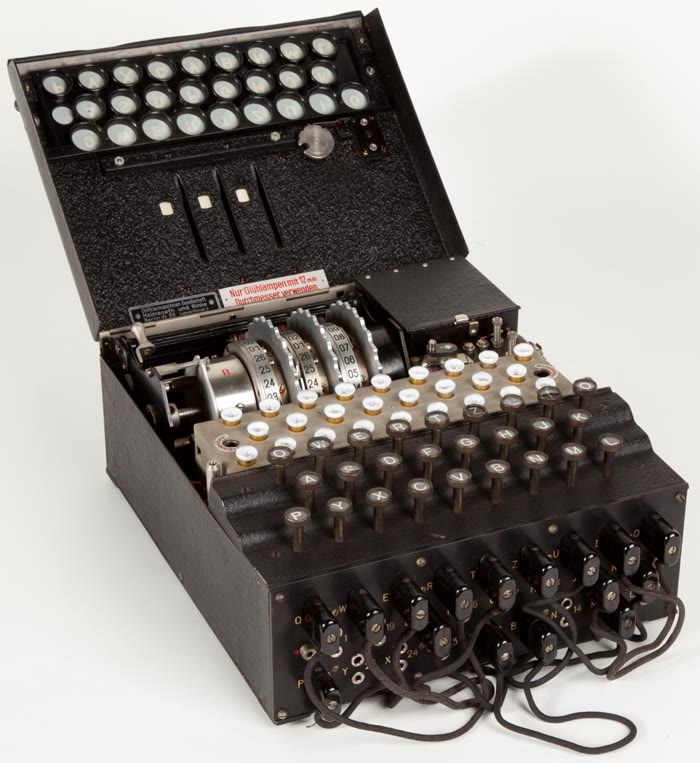
\includegraphics[width=0.36\linewidth]{images/book5/b3-27-enigma.jpg}}\hfill
\begin{minipage}{0.56\linewidth}\small
An Enigma I, the military model, in the Museo della Scienza e della Tecnologia, Milan (photograph by Alessandro Nassiri, 2012, CC BY-SA 4.0). The machine was invented by the German engineer Arthur Scherbius at the end of the First World War; its rotors scramble the 26 letters anew at each key press. % ledger: b3:enigma
\end{minipage}
\end{omfigure}

\section{Exercises}\label{sec:b3:symmetric-cryptography:exercises}

\begin{exercise}[$\star$]\label{exo:b3:symmetric-cryptography:1}
A \omterm{def:b3:symmetric-cryptography:otp}{one-time pad} on bytes encrypts the message \code{1011 0110} with the key \code{0110 1100}. Give the ciphertext, and the key that would make the same ciphertext decrypt to \code{0000 1111}.
\end{exercise}

\begin{exercise}[$\star$]\label{exo:b3:symmetric-cryptography:2}
A message of four blocks has $P_1 = P_3$. In which of ECB, CBC and CTR is $C_1 = C_3$? Under a fixed key, the same message is encrypted twice: in which modes are the two ciphertexts equal, if the IV or the counter is chosen afresh each time, and if it is reused?
\end{exercise}

\begin{exercise}[$\star$]\label{exo:b3:symmetric-cryptography:3}
How many 64-bit digests must be drawn, by the \omterm{thm:b3:symmetric-cryptography:birthday}{birthday bound}, for a collision to be more likely than not? About how many on average until the first? How long would a machine computing $10^9$ digests per second take?
\end{exercise}

\begin{exercise}[$\star$]\label{exo:b3:symmetric-cryptography:4}
Without running it, say what the line \code{c1 xor c2 = m1 xor m2} of \cref{out:b3:symmetric-cryptography:otp} contains at the positions where $m_1$ and $m_2$ have the same letter, and at the positions where one has a space and the other a capital letter.
\end{exercise}

\begin{exercise}[$\star\star$]\label{exo:b3:symmetric-cryptography:5}
\code{encrypt_buggy} in \code{exercises/ex5_ctr_bug.py} encrypts every message in \omterm{def:b3:symmetric-cryptography:modes}{CTR mode} from the counter block 0. Show what an eavesdropper learns from two messages, then fix it with an 8-byte \omterm{def:b3:symmetric-cryptography:stream}{nonce} per message in the first half of the counter block, sent with the ciphertext. How many messages, and how long, can one key then encrypt?
\end{exercise}

\begin{exercise}[$\star\star$]\label{exo:b3:symmetric-cryptography:6}
Write \code{cbc_decrypt_checked(key, iv, c)} from the definition of CBC and of PKCS\#7 \omterm{def:b3:symmetric-cryptography:modes}{padding}, using only \code{decrypt_block}. It must refuse an empty ciphertext, a length that is not a multiple of 16, and a bad \omterm{def:b3:symmetric-cryptography:modes}{padding}. Test it on the vector F.2.1 of SP 800-38A.
\end{exercise}

\begin{exercise}[$\star\star$]\label{exo:b3:symmetric-cryptography:7}
A letter-level \omterm{def:b3:symmetric-cryptography:otp}{one-time pad} shifts each letter of the message by a key letter, modulo 26. Prove that it has \omterm{def:b3:symmetric-cryptography:security}{perfect secrecy} when the key letters are independent and uniform. Then prove that the Vigenère cipher, which repeats a key of length $\ell$, does not, for messages longer than $\ell$.
\end{exercise}

\begin{exercise}[$\star\star$]\label{exo:b3:symmetric-cryptography:8}
Prove that $q$ uniform draws from $N$ values collide with probability at most $q(q - 1)/(2N)$. Together with \cref{thm:b3:symmetric-cryptography:birthday}, what do the two bounds say about $q = \sqrt{N}$?
\end{exercise}

\begin{exercise}[$\star\star$]\label{exo:b3:symmetric-cryptography:9}
With PKCS\#7 \omterm{def:b3:symmetric-cryptography:modes}{padding} and 16-byte blocks, how many blocks and \omterm{def:b3:symmetric-cryptography:modes}{padding} bytes do messages of 0, 1, 15, 16, 17 and 100 bytes produce? Why must a message of exactly 16 bytes get a whole block of \omterm{def:b3:symmetric-cryptography:modes}{padding}?
\end{exercise}

\begin{exercise}[$\star\star\star$]\label{exo:b3:symmetric-cryptography:10}
A service encrypts in \omterm{def:b3:symmetric-cryptography:modes}{CBC mode} with an IV that is the previous IV plus 1. In the \omterm{def:b3:symmetric-cryptography:security}{indistinguishability} game with chosen plaintexts, give an attacker that wins with probability 1, using one encryption after the challenge, and prove that it does. \code{exercises/ex10_iv_game.py} plays it.
\end{exercise}

\begin{exercise}[$\star\star\star$]\label{exo:b3:symmetric-cryptography:11}
Explain, from the structure of \omterm{def:b3:symmetric-cryptography:mac}{HMAC} with a Merkle--Damgård hash, why knowing $\mathrm{HMAC}(K, m)$ does not let an attacker compute $\mathrm{HMAC}(K, m \,\|\, \mathit{pad} \,\|\, m')$ by length extension. Which part of the computation would the attacker need, and why is it hidden?
\end{exercise}

\begin{exercise}[$\star\star\star$]\label{exo:b3:symmetric-cryptography:12}
Implement Poly1305 from RFC 8439, section 2.5: clamp $r$, then for each 16-byte block, with a byte \code{01} appended, add it to the accumulator and multiply by $r$ modulo $2^{130} - 5$; add $s$. Pass the test vector of section 2.5.2. Why must a Poly1305 key never authenticate two messages?
\end{exercise}

\section{Weekend problem}\label{sec:b3:symmetric-cryptography:problem}

\begin{problem}[{Weekend problem --- Collisions in the library's short checksums}]\label{pb:b3:symmetric-cryptography:1}
The library labels each catalogue record with a 32-bit checksum, the first 4 bytes of the record's SHA-256, and uses it to find duplicates: two records with the same checksum are assumed to be the same. The program below hashes records until two checksums collide, in 200 runs.

\omcode{code/bachelor-3/27-symmetric-cryptography/listings/birthday.py}{8}{17}{Hash numbered records until a checksum repeats.}\label{lst:b3:symmetric-cryptography:birthday}

\omoutput{code/bachelor-3/27-symmetric-cryptography/outputs/birthday.txt}{Two hundred runs: the first collision comes after 78,631 records on average, within 5\,\% of $\sqrt{\pi/2 \cdot 2^{32}}$.}\label{out:b3:symmetric-cryptography:birthday}

\needspace{4\baselineskip}\medskip\noindent\textbf{Part I --- The birthday bound.}
\begin{enumerate}
  \item How many different checksums are there?
  \item Write the probability that $q$ records all have different checksums, assuming checksums uniform and independent.
  \item Bound it with \cref{thm:b3:symmetric-cryptography:birthday} for $q = 10{,}000$ and $q = 100{,}000$.
  \item For which $q$ is a collision more likely than not?
  \item Why is the bound about $\sqrt{N}$ and not $N$?
  \item Is SHA-256 truncated to 32 bits still collision resistant? Preimage resistant?
\end{enumerate}

\needspace{4\baselineskip}\medskip\noindent\textbf{Part II --- Expected tries.}
\begin{enumerate}[resume]
  \item What mean does $\sqrt{\pi N / 2}$ give for $N = 2^{32}$?
  \item Explain why the runs vary so much, from 1,524 to 205,266.
  \item Two hundred runs average 78,631. How far is that from the formula, in per cent?
  \item With 20 runs instead of 200, how much larger would the typical error of the mean be?
  \item The library has 60,000 records. What is the chance that two share a checksum?
  \item What happens in the library's catalogue when they do?
\end{enumerate}

\needspace{4\baselineskip}\medskip\noindent\textbf{Part III --- Measured collisions.}
\begin{enumerate}[resume]
  \item Check from \cref{out:b3:symmetric-cryptography:birthday} that run 0's two records do share a checksum, and say how a reader can check it.
  \item Why are the records numbered with the run number in them?
  \item Would collisions come sooner if the records were short, or if they were long?
  \item The program keeps every checksum seen in a dictionary. How much memory does a run of 100,000 records take, roughly, and how could a collision be found with almost none?
  \item If an attacker can choose records, how does that change the risk?
  \item Could the library detect a duplicate safely with these checksums, and how?
\end{enumerate}

\needspace{4\baselineskip}\medskip\noindent\textbf{Part IV --- How many bits.}
\begin{enumerate}[resume]
  \item For $10^9$ records and a $b$-bit checksum, give the collision probability approximately.
  \item How many bits make it at most one in a million?
  \item What is it with 64 bits?
  \item Why is 128 bits the usual recommendation, rather than the minimum of question 20?
  \item What would SHA-256 in full cost the library in storage for $10^9$ records, against 4 bytes?
  \item Sum up: when does the first collision come for 32 bits, how close was the measurement, and how many bits does a catalogue of $10^9$ records need?
\end{enumerate}
\end{problem}
